\documentclass[border=10pt]{standalone}
\usepackage{pgfplots}
\pgfplotsset{compat=1.18}
\usepgfplotslibrary{fillbetween}
\begin{document}
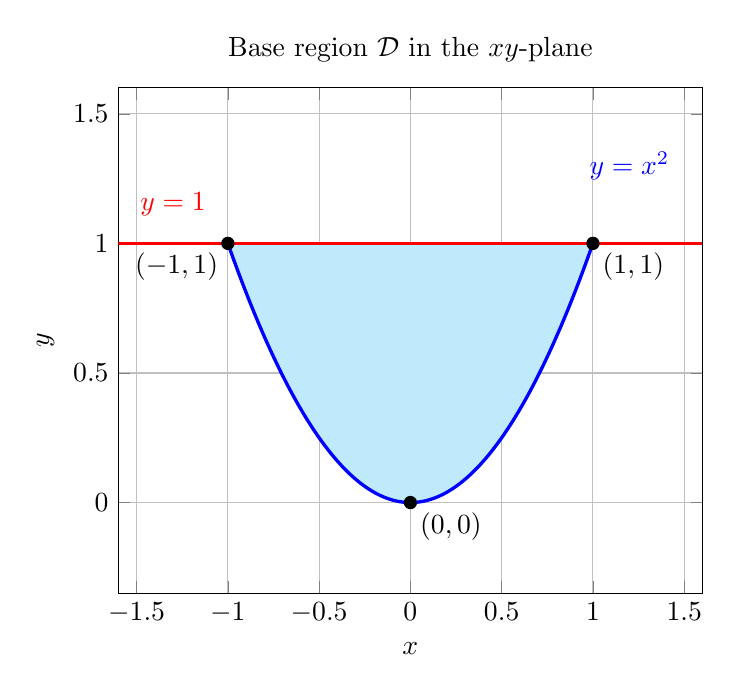
\begin{tikzpicture}
\begin{axis}[
    width=9cm, height=8cm,
    xmin=-1.6, xmax=1.6, ymin=-0.35, ymax=1.6,
    xlabel={$x$}, ylabel={$y$},
    title={Base region $\mathcal{D}$ in the $xy$-plane},
    grid=both, samples=200,
]
\addplot[name path=par, blue, very thick, domain=-1:1] {x^2};
\addplot[name path=line, red, very thick, domain=-1.6:1.6] {1};
\addplot[cyan!25] fill between[of=par and line, soft clip={domain=-1:1}];
\node[blue] at (axis cs:1.2,1.3) {$y=x^2$};
\node[red]  at (axis cs:-1.3,1.15) {$y=1$};
\addplot[only marks, mark=*, mark size=2.2pt, black] coordinates {(-1,1) (1,1) (0,0)};
\node[below left]  at (axis cs:-1,1) {$(-1,1)$};
\node[below right] at (axis cs:1,1) {$(1,1)$};
\node[below right] at (axis cs:0,0) {$(0,0)$};
\end{axis}
\end{tikzpicture}
\end{document}
